\documentclass[thesismargins, english, thesislinespacing, twoside, openright, upjsfrontpage]{rnthesis}
\usepackage[english]{babel}
\usepackage[T1]{fontenc}
\usepackage[utf8]{inputenc}
\usepackage{lmodern}

\usepackage{rnt-pic}
\usepackage{rnt-thm}

\usepackage{pdfpages} % inserting pdf pages

\usepackage[hyphens]{url} % format and linebreak of URLs

\usepackage{tikz}
\usetikzlibrary{datavisualization}
\usetikzlibrary{datavisualization.formats.functions}

\title{Replacing handwritten signatures with open electronic signature software}
\author{Jakub Ďuraš}
\typprace{bachelor's}
\rok{2020}
\odbor{Applied Informatics}
\miesto{Košice}
\podakovanie{
  Thanks to the Planet!
}
\veduci{RNDr. Viliam Kačala}
\pracovisko{Institute of Computer Science}
\pdfzadanie{zadanie.pdf}

\abstract{
With the recent changes in the legal status of electronic signatures in many parts of the world, there is a need for easily accessible solutions intended as an alternative to handwritten signatures. This may be more necessary than ever since electronic communication is the preferred way of communication. This bachelor thesis aims to explore the principles and legal status of electronic signatures, review current electronic signature software, and explore possible obstacles the open-source community is facing to develop such specialized applications. We propose an open-source, cross-platform, and user-friendly software compliant with the eIDAS Regulation (Regulation No 910/2014). Our application should allow ordinary users to quickly sign and verify signatures of different types of documents and therefore easily use them in everyday life.
}

\keywords{electronic signature, electronic seal, qualified, open-source, XAdES, PAdES, CAdES, desktop software}

\abstrakt{
Abstrakt v SK jazyku bude pridaný neskôr ako voľný preklad z EN verzie (pozri ďalšiu stranu). Predíde sa tak zbytočnej práci keďže EN abstrakt sa môže časom meniť.
}

\klucoveslova{elektronický podpis, elektronická pečať, kvalifikovaný, open-source, XAdES, PAdES, CAdES, počítačový softvér}

\bibliographystyle{alpha}

\begin{document}
\maketitle
\newpage
\tableofcontents
\listoffigures
\listoftables
% zoznam značiek a skratiek. Pre tento koncept neexistuje
% LaTeXovsky príkaz

\uvod

Will be added at the end. Lorem ipsum dolor sit amet, consectetuer adipiscing elit.
Integer lacinia, nulla porta varius tempus, lacus metus blandit
lorem, a rutrum justo wisi id sapien. Integer risus libero,
feugiat eleifend, ornare ac, volutpat nec, sem. In facilisis,
quam eu elementum aliquet, lorem quam euismod dui, aliquet
laoreet purus ipsum ac quam.

\chapter{Background and theory}

In our work, we rely on knowledge in several different subjects that we go over in the following sections.
TODO: Sounds very meh for the very first sentece of the thesis.
Firstly, the current state of the law and recent changes relating to the use of electronic signatures.
Secondly, on the well-established concepts in cryptography like asymmetric cryptography or hashing.
Lastly, expertise from the field of software engineering - especially design, implementation, and maintenance of computer software.
All in relation to the electronic signatures, and, where applicable, open-source and desktop computer software.

TODO: Think about adding section on handwritten signatures

\section{Law}

Unless specified otherwise, we are considering law applicable locally in the Slovak Republic (SR).
Its law is greatly influenced by the European Union (EU), being its member since 2004, and to some extent by the rest of the world.
Therefore, we can assume this is at least partially applicable outside of the SR.

\subsection{Signatures}

Signatures are essential part of the written legally binding documents like contracts.
They are permanently affixed to the document and are supposed to uniquely identify the person and its deliberate, informed consent.
As can be seen in the Slovak Civil Code, "A written legal act is valid if signed by the acting person;" \cite{civilcode}.
Law often explicitly requires signatures and further clarifies their expected use.
For example, when selling an enterprise, "The contract requires written form and attested signatures of the seller and the buyer." \cite{civilcode}.

Signature is considered an "attested signature"\footnote{Translation from "osvedčený podpis" as used in the Slovak law.} if it is attested by the authorized third party.
Such process, known as legalization, is regulated by the law and its purpose is to attest information which could form the basis for the exercise of rights or which could cause legal consequences \cite{notarylaw}.

With regards to electronic signatures, law within the EU used to differ, with law applicable in the SR being now repealed "Act No. 215/2002 Coll.".

\subsection{EU Regulation eIDAS} \label{eidas}

With intention to stimulate digital growth by building trust, the EU established regulation on electronic identification and trust services for electronic transactions in the internal market (eIDAS).
It applies from 1st of July 2016, replaces local law, and regulates, among other things, electronic signatures and its more specific variants.

\obrazok{./figures/electronic-advanced-qualified}{The relation between electronic, advanced, and qualified signatures.}{signature-comparison}

In general, electronic signature can be represented in different ways (e.g. as an image, text or other data attached to the document) and they \textbf{can not be denied in legal proceedings} just because they are in the electronic form \cite{eidas}.

Advanced electronic signatures are a subset of electronic signatures that have to \textbf{uniquely link and identify} the signature author, be created in a way that is \textbf{possible only by them} and any \textbf{changes to the signed document have to be detectable} \cite{eidas}.
From the technical point of view, standards PAdES, XAdES, and CAdES specified by the European Telecommunications Standards Institute (ETSI) comply with these requirements. We explain why this is the case in Chapter \ref{cryptography}.

Qualified electronic signatures (QES) are a subset of advanced electronic signatures with more specific requirements that can be found in the annex 1 of the eIDAS regulation\footnote{Available at https://eur-lex.europa.eu/legal-content/EN/TXT/HTML/?uri=CELEX:32014R0910\#d1e32-111-1.}.
In more practical terms, such advanced electronic signatures are created with a qualified device using a qualified certificate and a qualified trust service. Qualified in this case means authorized for such use by the legal authorities.

Furthemore, a qualified electronic signature has the legal effect of a handwritten signature \cite{eidas} and attested handwritten signatures in the SR.

Mentioned terminology is used when considering natural person. Legal entities are able to use "electronic seals", which are, from the technical point of view and our purposes, identical.

Overall, electronic signatures are supposed to be, within the EU, interoperable and transparent alternative to hand-written signatures.

\subsection{Software copyright}

Computer programs and associated materials are historically protected under copyright as literary works, and protected authors should be able to authorize or prohibit certain acts \cite{eeccopyright}.

Such right can be exercised, as far as we are concerned, to license the software under either proprietary or open-source license.
Proprietary meaning under exclusive legal right of the author, typically also confidential and distributed as a paid product.
Open-source meaning having its source code freely available, typically also distributed for free and without any liability (the software is provided "as is").

Motivation to license the software under an open-source license can differ, and so do such licenses.
While a proprietary license is usually made specifically for that entity and its interests, open-source licenses tend to be reused between different authors.
This means consumers of the software can quickly recognize their rights and responsibilities if they decide to use, modify, or distribute the software.
In general, we can classify the open-source licenses into two categories: permissive and copyleft.

Copyleft license, in general, requires the user to publish the modified work under the compatible (free) license.
Meaning forcing them to extend the rights they have received onto others and, in turn, somehow hindering use in software licensed under a different license.
Popular example of such license is the GNU General Public License (GPL) and its derivatives like GNU Lesser GPL (LGPL) or GNU Affero GPL (AGPL).

Permissive license, on the other hand, does not have such requirement in place and is more suitable for potential commercialization.
They typically allow commercial use, modifications, distribution or sublicensing as long as the author is not held liable and the original copyright and license is distributed with the software.
Often used permissive licenses are MIT License, Apache License or BSD License.

It is not uncommon to see hybrid licensing - licensing under more than one license, with one being typically open-source and one proprietary.
In this scenario, users can choose which license they want to use based on their needs.

\obrazok{./figures/license-comparison}{Classification and comparison of software licensing models.}{license-comparison}

As we have already mentioned, software licenses can influence whether and how it can be used as a part of different software.
Both when we are using someone else's software and when someone else is using our software.
Generally speaking, the more open the license is, the higher the probability it will not stop adoption for legal reasons.
Various possible combinations can be seen in Figure \ref{fig:license-compatibility}, where greyed out options mean such combination is not possible unless a separate licensing agreement is reached with the copyright owner.

\obrazok{./figures/license-compatibility}{Schematic representation of license directionality.\cite{licensing}}{license-compatibility}

\section{Cryptography} \label{cryptography}

Previously mentioned standards PAdES, XAdES, and CAdES define how asymmetric cryptography, hashing, or timestamping should be used to comply with the standards.
We go over a few of these topics and why they are able to satisfy the requirements.

\subsection{Asymmetric cryptography}

There are several issues that make symmetric encryption unsuitable. Let us imagine we are creating a key for each pair of users in our network - imaginary country Isle of Alice and Bob - for symmetric encryption and decryption of documents shared between each Alice and Bob.

\textbf{Secure distribution of keys} seems to be feasible when we are adding a new user to our network. We require each user to personally come and pick up physical device that contains pregenerated keys. Changes made after that, however, would mean we either need to require periodic personal visit to update the saved keys or transmission of these keys over some medium which can be potentialy unsafe. Any new members of the network are unable to participate untill other Alices and Bobs get their updates.

Even if we think we have established a reasonably secure way to do that and we are willing to wait, we realize the \textbf{number of keys} is quickly increasing with each new member. With \textit{n} users, the number of keys is

$$\frac{n \cdot (n - 1)}{2}$$

which means that even our little country with a population of only 70 000 requires roughly 2.5 billion keys. However, since our signature system needs to be portable, we will need to count also with a population of other EU countries, and the number of keys quickly explodes.

\begin{figure}[!htb]
  \centering

  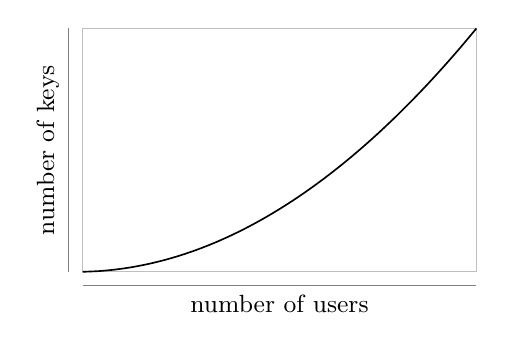
\begin{tikzpicture}
    \datavisualization [scientific axes=clean, visualize as smooth line, all axes={ticks={major={at={}}}}, y axis={label={number of keys}}, x axis={label={number of users}}]
    data [format=function] {
      var x : interval [2:125];
      func y = \value x*\value x;
    };
  \end{tikzpicture}

  \centerline{\parbox{13cm}{\sl \caption{Cubic growth of the number of keys.}}}
\end{figure}

\textbf{Either party can also lie} about not signing the document.
Since both have the key that can be used for encryption, they can sign any document on behalf of the other party, and there is no way to disprove it if we look at it as a third party.

These issues can be addressed with asymmetric cryptography.
In general, we assign a pair of keys to each person, one of them used for encryption (public key), another used for decryption (private key).
One party can encrypt, and the other is the only one that can decrypt.

Digital signatures are a specific public-key algorithms.
The signer is the only one who poses private key used for signing, and others can use the public key for verifying of signatures as can be seen in Figure \ref{fig:pubkey-scheme} where \(x\) is the "document", and \(s\) is the signature that is sent with the document.
Alice can then sign the document \textit{including} Bob's signature.

\obrazok{./figures/digital-signature-scheme}{Principle of digital signatures which involves signing and verifying a message (Paar 2009). TODO: I don't have rights to this image!!!}{pubkey-scheme}

Practical, widely used implementation of this idea is the RSA signature scheme that relies on the integer factorization problem (difficulty of factoring a product of two large primes) published in 1978 \cite{rsa}.

In Slovakia, the private key is usually handed over to the user personally, saved on the ID card. This ID card (used together with a card reader) provides an API for safe access, management, and cryptoprocessing. Such device is in general called a Hardware Security Module (HSM), and the API relevant for this thesis is PKCS \#11 \footnote{PKCS \#11 specification available at \url{http://docs.oasis-open.org/pkcs11/pkcs11-base/v2.40/os/pkcs11-base-v2.40-os.html}.}.

We are left with the problem of public key distribution - even though public-key schemes do not require a \textit{secure channel}, they require \textit{authenticated channels} for the distribution of the public keys \cite{cryptotxtbook}.

Common solution is the use of \textit{certificates}. Certificates are essentially digital signatures with metadata that can be used to establish validity of the received public key before it is used.
Distribution of such certificates is the responsibility of a Certification Authority (CA) - a third party that all users in the network trust. In the case of the Slovak ID cards, it is Disig - SVK eID ACA issued by the National Security Authority (NBÚ in Slovak).
Such certificates therefore reliably uniquely link and identify the public key owners as can be seen in Figure \ref{fig:certificate-scheme}\footnote{Created by unknown author, licensed under the CC BY-SA 3.0 license.}.

\obrazok{./figures/certificate-scheme}{Application of digital signature with certificate. TODO: Modify to add CA, remove hashing}{certificate-scheme}

Commonly used standard for public key certificates is X.509\footnote{Specification available under RFC5280 at \url{https://tools.ietf.org/html/rfc5280}.}.

\subsection{Hashing}

It is often useful to map data of arbitrary size to fixed-length (typically short) set of bits. This process is commonly called \textit{hashing}, function that can be used for it \textit{hash function}, and output of such function \textit{hash}.

In cryptography, we are considering only hash functions that can also satisfy these additional requirements:

\begin{enumerate}
  \item Deterministic - same input data are always mapped to the same hash.
  \item One-way - it should be practically impossible to retrieve input data for a given hash.
  \item Resistant to collisions - it should be practically impossible to find two inputs with the same hash.
  \item Even small change to the input should lead to significantly different hash - so-called \textit{avalanche effect}.
\end{enumerate}

In the context of digital documents, we can use such hash function to generate a hash for the document.
This hash can represent a document of any size and is used during the creation of a digital signature instad of document itself.
Any further changes to the document will, therefore, lead to a significantly different hash, which means the digital signature will no longer be valid, and these changes are detected.
For this purpose, only hash functions that are reasonably fast can be used, so that we can utilize them on documents of variable size.

TODO: Add scheme of document > hash - valid signature, change in document > different hash - invalid signature.

An example of commonly used hash function family is Secure Hash Algorithms (SHA), with hash functions relevant to this thesis being mainly SHA-2\footnote{SHA-2 specification available in FIPS PUB 180-4 at \url{https://nvlpubs.nist.gov/nistpubs/FIPS/NIST.FIPS.180-4.pdf}.}.

\subsection{Timestamping}

A common part of the paper signed documents is the date when they were signed.
Their digital counterpart is PKI-based \textit{trusted timestamping} - a process of digitally signing date and time of document creation or modification.
No one should be able to tamper with such timestamp - not even the author of the document.
Additionally, we should not be able to choose arbitrary date and time ourselves, but it should represent the actual time at the signing.

To achieve this, a trusted third party - Timestamping Authority (TSA) - is the one that will sign the hash of the document together with the current date and time.
This process can be seen in Figure \ref{fig:trusted-timestamping}\footnote{Schema created by Bart Van den Bosch, licensed under the CC BY-SA 2.0 BE license.}.
Verifying can be by decrypting this information using the public key and comparing the hashes. Any attempt at tampering is therefore detected.

\obrazok{./figures/trusted-timestamping}{Setting a timestamp via a trusted third party.}{trusted-timestamping}

The commonly used standard for the PKI-based timestamping is part of the X.509\footnote{Specification available under RFC3161 at \url{https://www.ietf.org/rfc/rfc3161.txt}.}.

\subsection{PAdES, XAdES, and CAdES}

Extensions for PDF files, XML files, and CMS signed data for signing using advanced electronic signatures (as explained in Chapter \ref{eidas}), are PAdES, XAdES, and CAdES, respectively.
They are defined in the respective specifications by the ETSI \footnote{Specification for PAdES is available at \url{https://www.etsi.org/deliver/etsi_ts/102700_102799/10277801/01.01.01_60/ts_10277801v010101p.pdf}} \footnote{Specification for XAdES is available at \url{https://uri.etsi.org/01903/v1.3.2/ts_101903v010302p.pdf}} \footnote{Specification for CAdES is available at \url{https://www.etsi.org/deliver/etsi_ts/101700_101799/101733/02.01.01_60/ts_101733v020101p.pdf}}.

When using PAdES, signatures are always part of the PDF file itself. This differs from XAdES, where the signature can be either part of the XML or provided as a separate file, or CAdES where signature is always in the form of binary data and it is up to the software.

All of them support multiple signatures applied in succession. Implementation of the PAdES is rather portable since any compatible PDF file reader or editor will work with the signatures in a similar way - signature created in one should be easily verifiable in any other. XAdES and CAdES, however, are usually tied to specific implementation or standard that is built on top of them.

\begin{table}[h!]
  \begin{tabular}{ |p{2cm}||p{2.2cm}|p{2cm}|p{3cm}|p{3.9cm}| }
    \hline
    Standard & Usable with & Format & Multi-signature & Appearance \\
    \hline
    PAdES & PDF                  & embedded         & yes, sequential    & supported            \\
    XAdES & XML, any             & XML              & yes                & depends on the usage \\
    CAdES & any                  & binary           & yes                & depends on the usage \\
    \hline
  \end{tabular}

  \caption{Overview of standards PAdES, XAdES, and CAdES}
  \label{table:1}
\end{table}

The ability to retain signed documents for a prolonged period of time is covered in these standards under optional Long-Term Validation (LTV) that allows archiving of documents for many years, possibly decades.
If enabled, a trustworthy timestamp is required as validity is verified for the time the signature (and therefore timestamp) was created.
The expiration time is then limited by the validity of the timestamp certificate.

\section{Software engineering}

TODO: Give definition to the software engineering, what aspects we are going over, our focus on the engineering relevant for the open source.

\subsection{Design}

TODO: System modeling

TODO: Architectural design

TODO: Design patterns

TODO: Dependability and Security

\subsection{Implementation}

TODO: Requirements engineering

TODO: Software reuse

TODO: Agile software development

\subsection{Testing and Releasing}

TODO: Quality management

TODO: Automated tests (pyramid, V-model)

TODO: Building, Release management

\subsection{Maintenance}

TODO: Evolution processes

TODO: OSS Sustainability

\chapter{Goals}

\section{Software}

TODO: Basis can be formed on the requirements article https://github.com/durasj/octosign/wiki/Initial-Requirements

TODO: Basic software requirements and more specific software requirements.

TODO: Enginnering parts - architecture, testing, maintainability.

TODO: Backends

\section{Information}

TODO: Website - multilingual, editable by the community
TODO: Global status - world map

Lorem ipsum dolor sit amet, consectetuer adipiscing elit.
Integer lacinia, nulla porta varius tempus, lacus metus blandit
lorem, a rutrum justo wisi id sapien. Integer risus libero,
feugiat eleifend, ornare ac, volutpat nec, sem. In facilisis,
quam eu elementum aliquet, lorem quam euismod dui, aliquet
laoreet purus ipsum ac quam.

\chapter{Analysis}

\section{Review of existing software}

TODO: Explain how they were picked, list them with info on the considered trait.

TODO: Maybe add a simple comparison table? Consider: - format support, commercial, localization, eIDAS, web, required setup, advanced features

\subsection{Desktop application JSignPdf}

\subsection{Web application zep.disig.sk}

\subsection{PDF viewer Adobe Acrobat Reader DC}

\subsection{Commercial desktop application D.PDF Signer}

\section{Modularity}

TODO: Rough overview of different ways modular architecture can be achieved. Focus on modularity via multiple independant applications.

\subsection{Communication}

TODO: Communication in multiple independant applications - IPC, Sockets, Pipes, STDIO.

\subsection{Bundling}

\subsection{Communicating and bundling with GPL software}

\chapter{Results}

\section{Desktop software}

TODO: Structure shoul roughly follow goals

Lorem ipsum dolor sit amet, consectetuer adipiscing elit.
Integer lacinia, nulla porta varius tempus, lacus metus blandit
lorem, a rutrum justo wisi id sapien. Integer risus libero,
feugiat eleifend, ornare ac, volutpat nec, sem. In facilisis,
quam eu elementum aliquet, lorem quam euismod dui, aliquet
laoreet purus ipsum ac quam.

\subsection{Comparison with existing software}

TODO: Reference table from analysis, add new column

\section{Website}

TODO: Structure shoul roughly follow goals

Donec dolor arcu, posuere at, vehicula vitae, accumsan ut,
lacus. Nulla tristique eros eu diam. Vivamus nec tortor vel
ligula elementum lacinia. Curabitur euismod eros adipiscing
ipsum. Donec sed quam at felis suscipit egestas. Morbi faucibus
libero sit amet libero. Nullam laoreet ipsum eu eros. Donec in
diam. Ut facilisis eros vel leo. Nunc vitae mauris. Donec leo
erat, luctus porttitor, laoreet eget, facilisis non, erat.
Integer nec elit.

\zaver

Ut lobortis semper risus, non condimentum dui convallis ut. Nulla eget volutpat tellus. Vestibulum lobortis tincidunt massa eu rhoncus. Suspendisse luctus eu dui non vehicula. Vivamus elementum auctor felis, placerat maximus magna lobortis ut. Donec placerat sem a mi sagittis blandit. Maecenas pellentesque laoreet mauris, dictum viverra ante sodales sed. Nullam non ligula quis ante ultricies finibus non quis ex. Ut tempor vitae ipsum sed imperdiet. Fusce aliquam nisl sit amet nunc tempor convallis. Vivamus vehicula magna sit amet purus commodo, et tincidunt purus accumsan. Nulla velit dolor, lacinia nec scelerisque a, euismod a sapien.
%

%\renewcommand{\bibname}{Zoznam použitej literatúry}
\begin{thebibliography}{9}
  % Príklady popisu dokumentov citácií podľa systému meno a dátum (Harvardský systém)
  % ----
  % Varianty zápisov autorov:
  % [1] GUZANIN, Štefan, Robert SABOVČÍK a Pavol KAČMÁR. Priezviská vždy VEĽKÝMI PÍSMENAMI,
  %   priezvisko prvého autora je vždy pred menom, druhý a ďalší autor majú zápis
  %   Meno PRIEZVISKO
  % [2] Neuvádzať rodné mená autorov.
  % [3] Verzálky nie sú povinné, možno použiť aj iné indikatívnejšie označenie
  %
  % --- 
  % 1. Knižná publikácia (monografia, učebnica, zborník ...)
  %   1 autor

  %  ------
  % Law
  %  ------
  \bibitem{civilcode}
  \emph{Act No. 40/1964 Coll. Civil Code}

  \bibitem{notarylaw}
  \emph{Act No. 323/1992 Coll. Notary Law}

  \bibitem{eidas}
  \emph{REGULATION (EU) No 910/2014 OF THE EUROPEAN PARLIAMENT AND OF THE COUNCIL, OJ L 257, 28.8.2014, p. 73–114}

  \bibitem{eeccopyright}
  \emph{Council Directive 91/250/EEC of 14 May 1991 on the legal protection of computer programs, OJ L 122, 17.5.1991, p. 42–46}

  %  ------
  % Article
  %  ------
  \bibitem{licensing}
  \osoba{Morin, A.}, et al. 2012. A Quick Guide to Software Licensing for the Scientist-Programmer. In: \emph{PLoS computational biology} [online]. Volume 8, issue 7 [cit. 2020-01-27]. Available at: \url{https://journals.plos.org/ploscompbiol/article?id=10.1371/journal.pcbi.1002598}

  \bibitem{cryptotxtbook}
  \osoba{PAAR, Christof} and \osoba{Pelzl, Jan}, 2009. \emph{Understanding Cryptography - A Textbook for Students and Practitioner}. Berlin: Springer. ISBN 978-3-642-04100-6.

  \bibitem{cryptojoy}
  \osoba{ROSULEK, Mike}. \emph{The Joy of Cryptography} [online]. Oregon: School of Electrical Engineering \& Computer Science, Corvallis, Oregon, USA [cit. 2020-04-18]. Available at: \url{http://web.engr.oregonstate.edu/rosulekm/crypto/crypto.pdf}

  \bibitem{rsa}
  \osoba{RIVEST, R. L.}, \osoba{SHAMIR, A.}, and \osoba{ADLEMAN, L.}, 1978. \emph{A method for obtaining digital signatures and public-key cryptosystems}. In: \emph{Communications of the ACM, 21(2):120–126, February 1978.}

  \bibitem{law}
  \osoba{MASON, Stephen}, 2017. \emph{Electronic Signatures in Law: Fourth Edition}. London: University of London. ISBN 978-1-911507-01-7. Available at: \url{https://humanities-digital-library.org/index.php/hdl/catalog/view/electronicsignatures/1/86-1}

  \bibitem{sommerville}
  \osoba{SOMMERVILLE, Ian}, 2016. \emph{Software Engineering, 10th Edition}. Harlow: Pearson Education. ISBN 978-0-13-394303-0.

  \bibitem{oss}
  \osoba{FOGEL, Karl}, 2019. \emph{Producing Open Source Software} [online]. TODO: TODO. [cit. 2020-04-21]. Available at: \url{https://producingoss.com/en/index.html}

  \bibitem{osslicensing}
  \osoba{LAURENT, Andrew}, 2008. \emph{Understanding Open Source and Free Software Licensing}. Sebastopol: O’Reilly Media. ISBN 978-0596005818.

  \bibitem{eloquentjs}
  \osoba{HAVERBEKE, Marijn}, 2018. \emph{Eloquent JavaScript, 3rd Edition}. San Francisco: No Starch Press. ISBN 978-1593279509.

  \bibitem{ydkjs}
  \osoba{SIMPSON, Kyle}, 2020. \emph{You Don't Know JS Yet (book series) - 2nd Edition} [online]. Available at: \url{https://github.com/getify/You-Dont-Know-JS}

  %\bibitem{2}
  %\osoba{Beck, G.}, 2007. \emph{Zakázaná rétorika: 30 manipulatívních technik}. Preklad
  %\osoba{Pomikálová, M.}. Praha: Grada Publishing. ISBN 978-80-247-1743-2.
  %\bibitem{3}
  %\osoba{Vojčík, P.}, 2010. \emph{Občianske právo hmotné II.} 3. prep. a dopl. vyd. Košice: UPJŠ v Košiciach. ISBN 978-80-7097-817-7.
  %  2 autori
  %\bibitem{4}
  %\osoba{Šoltés, M.} a \osoba{Radoňák, J.}, 2013. \emph{Základné princípy laparoskopickej chirurgie.} Košice: UPJŠ v Košiciach. ISBN 978-80-8152-074-7.
  % 3 autori
  %\bibitem{5}
  %\osoba{Guzanin, Š.}, \osoba{Sabovčík, R.} a \osoba{Kačmár, P.}, 2004. \emph{Selected Chapters of Plastic and Reconstructive Surgery: vysokoškolské učebné texty}. Košice: Univerzita Pavla Jozefa Šafárika v Košiciach, Lekárska fakulta. ISBN 80-7097-557-1.
  % 4 a viac autorov
  %\bibitem{6}
  %\osoba{Nagyová, I.} et al. 2009. \emph{Measuring health and quality of life in the chronically ill}. Košice: Equilibria. ISBN 978-80-892-8446-7.
  % Elektronická kniha
  %\bibitem{7}
  %\osoba{Speight, J. G.}, 2005. \emph{Lange's Handbook of Chemistry} [online]. London: McGraw-Hill. [cit. 2009.06.10.] ISBN 978-1-60119-261-5. Dostupné na: \url{http://www.knovel.com/web/portal/basic_search/display?_EXT_KNOVEL_DISPLAY_bookid=1347&_EXT_KNOVEL_DISPLAY_fromSearch=true&_EXT_KNOVEL_DISPLAY_searchType=basic}
  % zborník
  %\bibitem{8}
  %\osoba{Bačkor, M.} a \osoba{Mihaličová, S.}, zost., 2013. \emph{Zborník príspevkov z konferencie 11. dni doktorandov experimentálnej biológie rastlín a 13. konferencie experimentálnej biológie rastlín} [online]. Košice: Univerzita Pavla Jozefa Šafárika v Košiciach, Prírodovedecká fakulta [cit. 2009-06-10]. ISBN 9788081520327. Dostupné na: \url{
  %  http://www.upjs.sk/public/media/5596/PF-Zbornik-prispevkov-konferencie-11-dni-doktorandov.pdf}
  %
  % 2. Časopis (ako celok)
  %\bibitem{9}
  %\emph{Thaiszia: Journal of Botany}. Košice: P.J.Safarik University, Botanic Garden, \mbox{1990--\ .} ISSN 1210-0420.
  %\bibitem{10}
  %\emph{Ikaros: elektronický časopis o informační bezpečnosti} [online], 2002. [Praha]: Ikaros. 1997--{} [cit. 2002-03-08]. Dostupné na: \url{http://www.ikaros.cz/}. ISSN 1212-5075.
  % Jedno číslo časopisu
  %\bibitem{11}
  %\emph{CHIP: magazín informačních technologií}, 2013. Praha: Burda Praha, roč. 23, říjen. ISSN 1210-0684.
  %  ------
  %  3. Príspevok v knihe/zborníku
  %  ------
  %\bibitem{12}
  %\osoba{Sabol, J.}, 2000. Jazyk ako ľudské posolstvo: (namiesto doslovu). In: \emph{O jazyku a štýle kriticky aj prakticky}. Prešov: Náuka, s. 149--159. ISBN 809676022X.
  %\bibitem{13}
  %\osoba{Tóthová, E.} a kol., 2013. A rare t(9,22,16)(q34,q11,q24) translocation in chronic myeloid leukemia for which imatinib mesylate was effective: a case report. In: \emph{XXVII. Olomoucké hematologické dny s mezinárodní účastí, 12.--14.5.2013, Olomouc: sborník abstrakt}. Olomouc: Univerzita Palackého v Olomouci, s. 75--76. ISBN 9788024434803.
  %  ------
  % 4. Článok v časopise
  %  ------
  %\bibitem{14}
  %\osoba{Beňačka, J.} et al., 2009. A better cosine approximate solution to pendulum equation. In: \emph{International Journal of Mathematical Education in Science and Technology}. Vol. 40, no. 2, p. 206--215. ISSN 0020-739X.
  %\bibitem{15}
  %\osoba{Dubayová, T.} et al., 2010. The impact of the intensity of fear on patient's delay regarding health care seeking behavior: a systematic review vyhľadaní zdravotníckej starostlivosti. In: \emph{International Journal of Public Health}. Vol. 55, no. 5, p. 459--468. ISSN 1661-8556.
  %\bibitem{16}
  %\osoba{Steinerová, J.}, 2000. Princípy formovania vzdelania v informačnej vede. In: \emph{Pedagogická revue}. Roč. 2, č. 3, s. 8--16. ISSN 1335-1982.
  %\bibitem{17}
  %\osoba{Hoggan, D.}, 2002. Challenges, Strategies, and Tools for Research Scientists. In: \emph{Electronic Journal of Academic and Special Librarianship} [online]. Vol. 3, no. 3 [cit. 2013-01-10]. ISSN 1525-321X. Dostupné na: \url{http://southernlibrarianship.icaap.org/content/v03n03/Hoggan_d01.htm}
  %\bibitem{18}
  %\osoba{Srbecká, Gabriela}, 2010. Rozvoj kompetencí studentů ve vzdělávání. In: \emph{Inflow: information journal} [online]. Roč. 3, č. 7 [cit. 2013-08-06]. ISSN 1802-9736. Dostupné na: \url{http://www.inflow.cz/rozvoj-kompetenci-studentu-ve-vzdelavani}
  %  ------
  % 5. Príspevok v zborníku na CD-ROM
  %  ------
  %\bibitem{19}
  %\osoba{Zemánek, P.}, 2001. The machines for ``green works'' in vineyards and their economical evaluation. In: \emph{9th International Conference: proceedings. Vol. 2. Fruit Growing and viticulture} [CD-ROM]. Lednice: Mendel University of Agriculture and Forestry, p. 262--268. ISBN 80-7157-524-0.
  %  ------
  % 6. Záverečné a kvalifikačné práce
  %  ------
  %\bibitem{20}
  %\osoba{Mikulášiková, M.}, 1999. \emph{Didaktické pomôcky pre praktickú výučbu na hodinách výtvarnej výchovy pre 2. stupeň základných škôl}: diplomová práca. Nitra: UKF.
  %\bibitem{21}
  %\osoba{Urdzík, P.}, 2007. \emph{Predikcia intrauterinnej rastovej retardácie a preeklampsie pomocou biochemických a ultrazvukových markerov}: dizertačná práca. Košice: UPJŠ v Košiciach.
  %  ------
  % 7. Výskumné správy
  %  ------
  %\bibitem{22}
  %\osoba{Baumgartner, J.} a kol., 1998. \emph{Ochrana a udržiavanie genofondu zvierat, šľachtenie zvierat}: výskumná správa. Nitra: VÚŽV.
  %  ------
  % 8. Normy
  %  ------
  %\bibitem{23}
  %STN ISO 690: 2012. \emph{Informácie a dokumentácia. Návod na tvorbu bibliografických odkazov na informačné pramene a ich citovanie}.
  %  ------
  %  ------
  % 10. Zákon
  %  ------
  %\bibitem{25}
  %\emph{Zákon č.131/2002 Zb. o vysokých školách a o zmene a doplnení niektorých zákonov.}
  %\bibitem{26}
  %\emph{Zákon č. 313/2001 o verejnej službe.}

\end{thebibliography}

\end{document}
